\documentclass[conference]{IEEEtran}
\IEEEoverridecommandlockouts
% The preceding line is only needed to identify funding in the first footnote. If that is unneeded, please comment it out.
\usepackage{cite}
\usepackage{amsmath,amssymb,amsfonts}
\usepackage{algorithmic}
\usepackage{graphicx}
\usepackage{textcomp}
\usepackage{xcolor}
\usepackage{hyperref}
\usepackage{listings}
\usepackage{float}
\usepackage{todonotes}

\def\BibTeX{{\rm B\kern-.05em{\sc i\kern-.025em b}\kern-.08em
    T\kern-.1667em\lower.7ex\hbox{E}\kern-.125emX}}

\newcommand{\arrowright}{$\,\to\,$}
    
\begin{document}

\title{App-controlled LEGO robotic arm\\
{\footnotesize Project of lecture ''Mobile Computing'' (winter term 2018/2019)}
}

\author{
\IEEEauthorblockN{Christoph Ulrich}
\IEEEauthorblockA{%\textit{dept. name of organization (of Aff.)} \\
\textit{HTWG Konstanz}\\
Constance, Germany\\
christoph.ulrich@htwg-konstanz.de}
\and
\IEEEauthorblockN{Benjamin Schaefer}
\IEEEauthorblockA{%\textit{dept. name of organization (of Aff.)} \\
\textit{HTWG Konstanz}\\
Constance, Germany\\
benjamin.schaefer@htwg-konstanz.de}
}

\maketitle

\begin{abstract}
it's reasonable to write this after all other sections of this paper have been completed
\end{abstract}

%\begin{IEEEkeywords}
%component, formatting, style, styling, insert
%\end{IEEEkeywords}\

\section{Introduction / Motivation}
\begin{itemize}
	\item control of a robotic arm is a fundamental task in robotics - easy hands-on experience for everybody to this fundamental robotic application with this paper and the created low cost LEGO 3-DoF (\textit{Degrees of Freedom}) robot arm  (incl. instructions)
	\item application and hardware could be used in basic lecture "Grundlagen der mobilen Robotik" to better understand robot kinematics, ROS and a bit of perception
	\item recycling of old and unused hardware of the robotics lab at the HTWG Konstanz
	\item typical industrial applications to control a robotic arm run on more powerful hardware and often offer a complicated and - for beginners - confusing GUI, \todo[author=Christoph, inline]{insert example(s)} so we developed an easy to use mobile application for Android platforms
	\item ROS because widely used, very modular/extensible and basic framework which almost every student starting with robotics has to get in touch with
\end{itemize}
\par

\todo[author=Christoph, inline]{new paragraph - description of background and main ''problem''}
\begin{itemize}
	\item which platform to choose for controlling the  arm and driving the motors (Arduino, Raspberry, etc.) - should consume as little energy as possible,  should be flexible and portable
	\todo[author=Christoph, inline]{note that in \ref{sec:platform}}
	\item another aspect \arrowright how should the application on the mobile device communication with the controlling device \arrowright BT, WiFi, (lost of steering commands due to radio lacks etc.)
	\item arm construction \arrowright not too many components, not too heavy so that the motors are able to drive the arm even with more than one joint and with gripper load (to demonstrate gripping)
	\item app \arrowright 
\end{itemize}
Constructing a robot arm generally leads to some difficulties.

\section{State of the Art}

\todo[author=Beide, inline]{find two or three example applications/hardware compontents, analyze and compare them, also look at mobile application programming techniques used in these works}
\begin{itemize}
	\item https://www.hackster.io/slantconcepts/control-arduino-robot-arm-with-android-app-1c0d96
	\item https://www.instructables.com/id/Robot-Arm-Arduino-App/
	\item https://www.kuka.com/en-us/products/robotics-systems/software/application-software/kuka-hrc-guide-app
\end{itemize}

\section{Proposed Approach}\label{sec:approach}

\subsection{Requirements Engineering}\label{sec:requirements}
\todo[author=Beide, inline]{what should the arm be able to achieve in the end? How should the app look like and which functions does it have to provide?}

\subsection{Platform Decision}\label{sec:platform}
\todo[author=Beide, inline]{Raspberry, Arduino, NXT, EV3, others?}

\subsection{Arm Construction}\label{sec:construction}
\todo[author=Benni, inline]{moment/transmission calculations, ... }

\subsection{Algorithms}\label{sec:algorithms}
\todo[author=Christoph, inline]{implementation of forward and backward kinematics }
\subsubsection{Kinematics}\label{sec:kinematics}
In order to control the arm it is essential to solve either it's forward or backward kinematics. For our application, we need both problems to be solved. Users of the application should be able to directly control each joint individually (forward kinematics) as well as to move the TCP into a desired position (backward kinematics). We will first take a look at the calculation of the forward kinematics and then introduce a short geometric solution of the backward kinematics for our 3-DoF arm.
\todo[author=Christoph, inline]{TCP - list of abbreviations may be necessary}
\todo[author=Beide, inline]{measurement of arm dimensions}
\par
The goal of forward kinematics is to determine the pose (position and orientation) of the TCP for a given set of joint angles. The pose of the TCP regarding the origin of the robot arm can be described as a concatenation of $n$ transformations, where $n$ is the number of joints, of which every one has its own coordinate system. For our case $n$ is 3:
\begin{equation}\label{eq:trans_matrix}
T_0^3 = T_0^1 * T_1^2 * T_2^3
\end{equation}
where $T_i^{i-1}$ is a transformation matrix according to the \textit{Denavit-Hartenberg} convention:
\begin{equation}\label{eq:dh-convention}
T_i^{i-1} = Tl(0,0,d_i) * R(z, \theta_i) * Tl(a_i,0,0) * R(x, \alpha_i)
\end{equation}
with $Tl$ being a translation matrix, $R$ a rotation matrix, $d_i$ a translation in z, $a_i$ a translation (for prismatic joints) in x, $\theta_i$ a rotation around z and $\alpha_i$ a constant tilt angle between both joints. In our case we don't use prismatic joints and there are no constant tilt angles between the joints (they are all variable). So equation \ref{eq:dh-convention} simplifies to 
\begin{equation}\label{eq:dh-convention-short}
T_i^{i-1} = Tl(0,0,d_i) * R(z, \theta_i)
\end{equation}
By solving equation \ref{eq:dh-convention-short} we get the following transformation matrix $T_i^{i-1}$ for the forward kinematics:
\[
\begin{matrix}
\cos(\theta_i) & -\sin(\theta_i) & 0 & l_i \cdot \cos(\theta_i)  \\
\sin(\theta_i) & \cos(\theta_i) & 0 & l_i \cdot \sin(\theta_i) \\
0 & 0 & 1 & 0 \\
0 & 0 & 0 & 1
\end{matrix}
\]
Finally, one generally can get the pose of the TCP in the world coordinate system (usually that means with reference to the coordinate system of the robot's base) by multiplying the concatenated transformation matrix \ref{eq:trans_matrix} built from the set of given joint angles $\theta_i$ and the known lengths of the arm parts $l_i$ with the origin of the base:
\begin{equation}\label{eq:tcp_goal}
p_{tcp} = T_0^3 * \begin{pmatrix}0\\0\\0\\1\end{pmatrix}
\end{equation}
Note that one have to use homogeneous coordinates here. Also one should remember that $p_{tcp}$ is the pose of the TCP-origin. Usually users want to get the gripping point of their tool - in this case just add the half of the gripper length to the x-direction to the vector in equation \ref{eq:tcp_goal}.
\\
\par

Vice versa, the goal of backward kinematics is to calculate a set of joint angles from a desired TCP-pose. $\chi$

\begin{itemize}
	\item generally for actual 3 dof
	\item visualization and control over 2 dof, separate control of base and gripper
\end{itemize}

\begin{figure}[htbp]
	\centerline{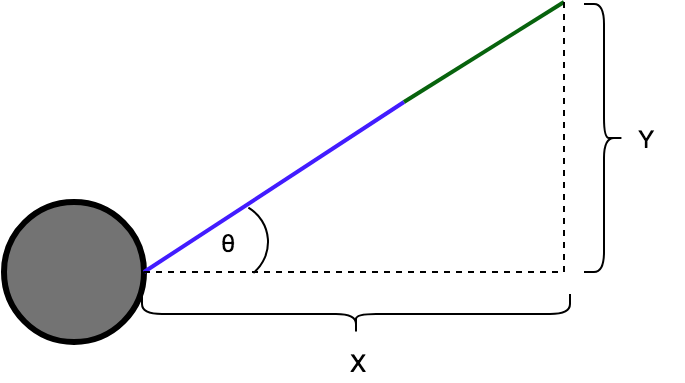
\includegraphics[scale=0.3]{img/kin_yaw_top_view.png}}
	\caption{Top view of the robot. Rotation angle of base joint can be easily calculated with the arctan.}
	\label{fig:yaw_calc}
\end{figure}

\begin{figure}[htbp]
	\centerline{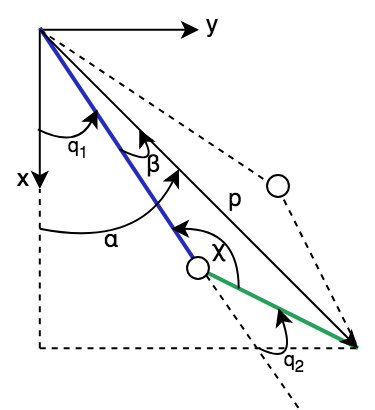
\includegraphics[scale=0.3]{img/kin_q1_q2.png}}
	\caption{Top view of the robot. Rotation angle of base joint can be easily calculated with the arctan.}
	\label{fig:q1_q2_calc}
\end{figure}

\subsection{App Development}\label{sec:development}
\todo[author=Christoph, inline]{communication/process description, ROS, navigation strategy, ... }

\subsection{Expected Results}\label{sec:expectedresults}
\todo[author=Christoph, inline]{speed, accuracy, ...}

\section{Results}

\section{Conclusion}

\section{Further Work}
\begin{itemize}
	\item 3D graphics in App
	\item EV3
	\item algorithms
	\item external better sensors to optimize
	\item ...
\end{itemize}


\begin{thebibliography}{00}
\bibitem{onlPrimitives} 
Khronos - OpenGL: Primitives - Triangle Primitives,
\\\texttt{https://www.khronos.org/opengl/wiki/Primitive}
\end{thebibliography}

\listoftodos

\end{document}